\documentclass{article}

% =========================
% NeurIPS 2026 Style
% =========================
\PassOptionsToPackage{numbers,sort&compress}{natbib}
\usepackage{neurips_2026}

\usepackage[utf8]{inputenc}
\usepackage[T1]{fontenc}

% =========================
% Typography / Layout
% =========================
\usepackage{microtype}
\usepackage{booktabs}
\usepackage{nicefrac}

% =========================
% Math
% =========================
\usepackage{amsmath, amssymb, amsthm, mathtools, bm}
\usepackage{amsfonts}
\DeclareMathOperator*{\argmax}{arg\,max}
\DeclareMathOperator*{\argmin}{arg\,min}

% =========================
% Figures / Tables
% =========================
\usepackage{graphicx}
\usepackage{subcaption}
\usepackage{float}

% =========================
% Algorithms
% =========================
\usepackage{algorithm}
\usepackage{algorithmic}

% =========================
% References / Links
% =========================
\usepackage[colorlinks=true,linkcolor=blue,citecolor=blue,urlcolor=blue]{hyperref}
\usepackage[nameinlink,noabbrev]{cleveref}

% =========================
% Colors (for TODO placeholders)
% =========================
\usepackage{xcolor}
\newcommand{\todo}[1]{\textcolor{red}{[TODO: #1]}}

% =========================
% Theorem Envs (NeurIPS-friendly)
% =========================
\theoremstyle{definition}
\newtheorem{definition}{Definition}
\newtheorem{assumption}{Assumption}

\theoremstyle{plain}
\newtheorem{theorem}{Theorem}
\newtheorem{lemma}{Lemma}
\newtheorem{proposition}{Proposition}
\newtheorem{corollary}{Corollary}

\theoremstyle{remark}
\newtheorem{remark}{Remark}

% =========================
% Custom Commands
% =========================
\newcommand{\NSW}{\mathcal{W}_{\mathrm{NSW}}}
\newcommand{\AVoI}{\mathcal{V}_{\mathrm{mask}}}
\newcommand{\E}{\mathbb{E}}
\newcommand{\KL}{D_{\mathrm{KL}}}
\newcommand{\ind}{\mathbb{I}}

% =========================
% Paper Meta
% =========================
\title{Computational Social Contract (CSC): Protocol-Level Collective Alignment in Heterogeneous Multi-Agent Systems via an Algorithmic Veil of Ignorance}

\author{%
  Anonymous Authors \\
  Affiliation \\
  Address \\
  \texttt{email} \\
}
\date{}

\begin{document}
\maketitle

\begin{abstract}
As AI systems transition from single agents to interacting collectives, alignment must extend from individual intent-following to \emph{collective} objectives that remain stable under heterogeneity, scarcity, and adversarial deviations.
We introduce the \textbf{Computational Social Contract (CSC)}, a protocol that (i) learns a \emph{contract policy} under an identity-blind \textbf{Algorithmic Veil of Ignorance (AVoI)} and a welfare objective that discourages near-zero outcomes, and (ii) stabilizes identity-aware execution via \textbf{KL grounding} and an \textbf{arbitration layer} trained against evasive deviations.
We propose \textit{Silicon Commune}, a scalable heterogeneous resource dilemma benchmark with controlled shock families and Byzantine stress tests.
Across strong CTDE baselines (VDN/QMIX/COMA and PPO-style centralized-critic variants), CSC improves equity (Gini $\downarrow$, Jain $\uparrow$) and robustness (shock survival $\uparrow$, Byzantine resilience $\uparrow$) while maintaining competitive throughput.
\end{abstract}

% =========================================================
\section{Introduction}
\label{sec:intro}

Multi-agent systems are increasingly deployed as \emph{collectives}: swarms of agents sharing resources, negotiating constraints, and affecting each other's outcomes \citep{dafoe2021cooperativeai_nature,rahwan2019machine}.
In such settings, naive efficiency maximization can produce \emph{polarization} and \emph{fragility}: strong agents exploit weak ones, drive some returns toward zero, and create single points of failure that collapse under shocks or strategic deviations \citep{leibo2017multiagent,hughes2018inequity,hardin1968tragedy,ostrom1990governing}.
This motivates \emph{collective alignment}: a design goal where cooperative behavior remains equitable and robust under heterogeneity and distribution shift \citep{christian2020alignment,russell2019humancompatible}.

A natural approach is to encode social welfare in the objective \citep{sen1973inequality,young1994equity}.
However, welfare-only training is insufficient when execution policies can deviate after learning, or when learning exploits identity-index shortcuts that do not generalize.
Moreover, in heterogeneous populations, identity features (endowments, capabilities) create incentives to specialize policies to privileged roles.
This gap suggests a protocol view: separate \emph{contract formation} (how the group agrees on a rule) from \emph{contract execution} (how individual policies behave when identities are real) \citep{sandholm1999distributed,shoham1995agent}.

\paragraph{Our approach.}
We propose \textbf{Computational Social Contract (CSC)}, a protocol with two phases:
(i) \textbf{Contract Formation} learns a contract policy under an \textbf{Algorithmic Veil of Ignorance (AVoI)} that suppresses identity-index information during learning, inspired by the ``original position'' \citep{rawls1971theory};
(ii) \textbf{Execution Grounding} trains identity-aware execution policies regularized toward the contract and stabilized by an \textbf{arbitration layer} that penalizes detected violations and is trained against evasive deviations \citep{myerson1981optimal,hurwicz2006design}.

\paragraph{Contributions.}
\begin{itemize}
  \item \textbf{Protocol-level formulation.} We formulate collective alignment as contract formation under AVoI plus identity-aware execution grounded by KL regularization and arbitration.
  \item \textbf{Implementable AVoI operators.} We define a family of masking operators (permutation/partial/noise) that induce symmetry and reduce identity-index shortcutting.
  \item \textbf{Benchmark and evaluation axes.} We introduce \textit{Silicon Commune} with controlled shock processes and Byzantine stress tests, and evaluate efficiency--equity--robustness jointly.
\end{itemize}

% =========================================================
\section{Related Work}
\label{sec:related}

\paragraph{Cooperative MARL and CTDE.}
Our baselines follow the CTDE paradigm \citep{oliehoek2016concise,bernstein2002complexity}, including value decomposition (VDN \citep{sunehag2017vdn}, QMIX \citep{rashid2018qmix}) and counterfactual policy gradients (COMA \citep{foerster2018coma}).
We build on Markov games and stochastic games foundations \citep{shapley1953stochastic,littman1994markov}.

\paragraph{Social dilemmas and fairness in MARL.}
Sequential social dilemmas formalize tensions between individual incentives and group welfare \citep{leibo2017multiagent}.
In inequity settings, intrinsic or shaped objectives can improve cooperation \citep{hughes2018inequity,jaques2019socialinfluence}.
CSC differs by separating \emph{contract learning} from \emph{execution enforcement}, and by explicitly suppressing identity-index information during contract formation.

\paragraph{Welfare objectives and resource allocation fairness.}
Nash bargaining and Nash social welfare connect efficiency with fairness by penalizing near-zero outcomes \citep{nash1950bargaining,kalai1975other}.
Classic inequality measures include the Gini coefficient \citep{gini1912variabilita} and Jain's index \citep{jain1984fairness}, and proportional fairness arises in network utility maximization \citep{kelly1997charging,mo2000fair}.
CSC uses welfare in contract formation and complements it with enforcement against deviations.

\paragraph{Robustness and adversarial deviations.}
Robust RL and adversarial training study stability under disturbances and adversaries \citep{pinto2017robust,behzadan2017vulnerabilities}.
In multi-agent systems, malicious or Byzantine behaviors are a classical threat model \citep{lamport1982byzantine}.
CSC operationalizes robustness by training an arbitration detector against evasive deviation policies and evaluating across shock families and Byzantine stress tests.

% =========================================================
\section{Problem Formulation}
\label{sec:problem}

We consider an $n$-agent Markov game with global state $s_t$, local observations $o_{i,t}$, joint action $a_t=(a_{1,t},\dots,a_{n,t})$, and per-agent reward $r_{i,t}$ \citep{shapley1953stochastic,littman1994markov}.
Each agent has an endowment/identity vector $\phi_i \in \mathbb{R}^d$ (capabilities, capacities, or costs) that affects rewards and transitions.

\paragraph{Objective: Nash Social Welfare.}
We adopt an $\epsilon$-stabilized Nash Social Welfare (NSW) objective:
\begin{equation}
\label{eq:nsw}
\NSW(\pi) \;=\; \frac{1}{n} \sum_{i=1}^n \log\!\big(\epsilon + \E_\pi[G_i]\big),
\end{equation}
where $G_i=\sum_{t=1}^T \gamma^{t-1} r_{i,t}$ is the episodic return.
NSW is a standard welfare criterion that balances efficiency and discourages near-zero outcomes \citep{nash1950bargaining,kalai1975other}.

\begin{proposition}[NSW discourages near-zero outcomes]
\label{prop:nsw_pareto}
Holding total return fixed, the NSW objective \eqref{eq:nsw} penalizes allocations that drive any $\E_\pi[G_i]$ toward zero more strongly than linear welfare, inducing an implicit inequality aversion.
\end{proposition}

% =========================================================
\section{Method: Computational Social Contract (CSC)}
\label{sec:method}

CSC separates \textbf{contract formation} from \textbf{execution}.
Contract formation learns a symmetric contract policy under identity masking.
Execution trains identity-aware policies regularized toward the contract and stabilized by an arbitration layer.

% ---------------------------------------------------------
\subsection{Algorithmic Veil of Ignorance (AVoI)}
\label{sec:avoi}

\begin{definition}[AVoI operator family]
Let $\Phi=\{\phi_1,\dots,\phi_n\}$ be the set of identity/endowment vectors.
AVoI produces masked identities $\bar{\phi}_i$ using a masking kernel $\mathcal{T}_\eta$:
\[
\bar{\phi}_i \sim \mathcal{T}_\eta(\phi_i;\Phi),
\]
where $\eta$ controls masking strength.
The masked observation is $o'_{i,t}=(o^{env}_{i,t}, \bar{\phi}_i)$.
\end{definition}

We implement three AVoI instances:
(i) \textbf{Permutation AVoI}: sample $\sigma \sim \mathrm{Unif}(\mathcal{S}_n)$ and set $\bar{\phi}_i=\phi_{\sigma(i)}$;
(ii) \textbf{Partial AVoI}: dropout mask $m\sim\mathrm{Bernoulli}(1-\eta)^d$ and $\bar{\phi}_i=m\odot\phi_i$;
(iii) \textbf{Noisy AVoI}: $\bar{\phi}_i=\phi_i+\epsilon$, $\epsilon\sim\mathcal{N}(0,\sigma^2 I)$.

\begin{proposition}[Permutation invariance of the masked objective]
\label{prop:perm_invariance}
Let $J(\pi)=\E_{\sigma}[\NSW(\pi;\sigma)]$ denote NSW under permutation AVoI.
Then $J(\pi)$ is invariant to relabeling agents, encouraging symmetric contract policies.
\end{proposition}

% ---------------------------------------------------------
\subsection{Two-phase training}
\label{sec:two_phase}

\paragraph{Phase I: Contract formation.}
Agents learn $\pi_{\text{contract}}$ on masked observations to maximize NSW:
\[
\max_{\theta_c}\; \NSW(\pi_{\text{contract}}(\cdot;\theta_c))\quad\text{under AVoI}.
\]

\paragraph{Phase II: Execution grounding.}
Agents learn identity-aware execution policies $\pi_{\text{exec}}$ on real identities, regularized toward the contract:
\begin{equation}
\label{eq:kl_ground}
\max_{\theta_e}\;\sum_i \E\!\left[G_i\right] \;-\; \beta \sum_i \E\!\left[\KL\big(\pi_{\text{exec}}(\cdot|o_{i,t})\;\|\;\pi_{\text{contract}}(\cdot|o'_{i,t})\big)\right],
\end{equation}
where $\beta$ controls contract adherence.

% ---------------------------------------------------------
\subsection{Arbitration layer: deviation proposer and detector}
\label{sec:arbitration}

CSC deters deviations with an arbitration detector $d_\omega(o,a)\in[0,1]$ trained to discriminate contract-compliant actions from deviations.
A deviation proposer $q_\psi(\cdot|o)$ searches for profitable/evasive deviations.
During execution, CSC shapes reward:
\begin{equation}
\label{eq:shaping}
r^{shaped}_{i,t} = r_{i,t} - \kappa\cdot \ind\!\big[d_\omega(o_{i,t},a_{i,t}) \ge \tau\big],
\end{equation}
with penalty scale $\kappa$ and threshold $\tau$ calibrated at a fixed false-positive rate (Appendix~\ref{app:detector}).
Reward shaping is grounded in classical theory \citep{ng1999policyinvariance} but here is tied to learned violation detection.

\begin{lemma}[Deviation success bound (informal)]
\label{lem:sdrbound_main}
If the arbitration penalty scale $\kappa$ exceeds the maximal achievable deviation advantage over horizon $H$, then the \emph{successful deviation rate} (SDR) is bounded by the detector's false-negative rate (FNR). Formal definitions and measurement protocol are in Appendix~\ref{app:metrics}.
\end{lemma}

\begin{algorithm}[t]
\caption{CSC (AVoI Contract + Grounding + Arbitration)}
\label{alg:csc}
\begin{algorithmic}[1]
\STATE Initialize contract policy $\pi_{\text{contract}}(\theta_c)$, execution policy $\pi_{\text{exec}}(\theta_e)$, proposer $q_\psi$, detector $d_\omega$.
\FOR{each iteration}
  \STATE Sample identity set $\Phi=\{\phi_i\}$ and AVoI mask (e.g., permutation $\sigma$).
  \STATE \textbf{Phase I (Contract):} rollout masked obs $o'_{i,t}$, update $\theta_c$ to maximize NSW \eqref{eq:nsw}.
  \STATE \textbf{Proposer/Detector:} update $q_\psi$ to find high-gain evasive deviations; update $d_\omega$ via balanced BCE (Appendix~\ref{app:detector}).
  \STATE \textbf{Phase II (Execution):} rollout real obs $o_{i,t}$, shape reward \eqref{eq:shaping}, update $\theta_e$ with objective \eqref{eq:kl_ground}.
\ENDFOR
\end{algorithmic}
\end{algorithm}

% =========================================================
\section{Experiments}
\label{sec:experiments}

\subsection{Benchmark: Silicon Commune (main summary)}
\label{sec:env_main}

We introduce \textit{Silicon Commune}, a heterogeneous resource dilemma designed to stress-test collective alignment under scarcity.
Each episode has shared resource $R_t$ and heterogeneous endowments $\phi_i=(c_i,m_i)$.
Agents choose extraction requests $a_{i,t}\in[0,1]$; realized allocations are proportional to attempted extraction under pool availability.
Rewards use diminishing returns $u_i(e)=\log(1+c_i e)$, plus action cost.
Resource shocks follow Bernoulli/Poisson/Markov families (Appendix~\ref{app:shock}), and Byzantine stress tests randomly replace a subset of agents with malicious policies (Appendix~\ref{app:byzantine}).

\begin{table}[t]
\centering
\caption{Silicon Commune main setting (full grids in Appendix).}
\label{tab:env_config}
\begin{tabular}{ll}
\toprule
Parameter & Value \\
\midrule
Agents $n$ & 100 \\
Episode length $T$ & 200 \\
Regen $\rho$ & 1.0 \\
Strong ratio & 0.1 \\
Strong $(c,m)$ & $[5,10]\times[5,10]$ \\
Weak $(c,m)$ & $[1,2]\times[1,2]$ \\
Action bins $K$ & 11 \\
Masking strength $\eta$ & 0.8 \\
\bottomrule
\end{tabular}
\end{table}

\subsection{Baselines and protocol}
\label{sec:baselines}

We compare against CTDE baselines: VDN \citep{sunehag2017vdn}, QMIX \citep{rashid2018qmix}, COMA \citep{foerster2018coma}, and a PPO-style centralized-critic baseline (clipped policy gradient with GAE) \citep{schulman2016gae}.
We match interaction budgets, parameter counts, and trial budgets (Appendix~\ref{app:hparam_search}).

\subsection{Metrics}
\label{sec:metrics}

We report:
\textbf{Efficiency} (Throughput, NSW),
\textbf{Equity} (Gini \citep{gini1912variabilita}, Jain \citep{jain1984fairness}),
\textbf{Robustness} (Shock survival / Resilience AUC, Byzantine resilience),
and \textbf{Deviation resistance} (DVR/SDR).
Definitions and computation details appear in Appendix~\ref{app:metrics}.

% =========================================================
\section{Results}
\label{sec:results}

\subsection{Main results}
\label{sec:main_results}

CSC improves equity and robustness while maintaining competitive efficiency.
\Cref{tab:main_results} reports throughput, inequality metrics, and Resilience AUC over shock sweeps.
Learning curves (NSW, Gini) appear in \Cref{fig:learning_curves}.

\begin{table}[t]
\centering
\caption{\textbf{Main results on Silicon Commune.} Mean$\pm$std over 5 seeds. Resilience AUC averages survival over shock sweep grids (Appendix~\ref{app:shock}).}
\label{tab:main_results}
\begin{tabular}{lcccc}
\toprule
Method & Throughput $\uparrow$ & Gini $\downarrow$ & Jain $\uparrow$ & Resilience AUC $\uparrow$ \\
\midrule
PPO-CTDE (centralized critic) & \todo{} & \todo{} & \todo{} & \todo{} \\
VDN \citep{sunehag2017vdn}    & \todo{} & \todo{} & \todo{} & \todo{} \\
QMIX \citep{rashid2018qmix}   & \todo{} & \todo{} & \todo{} & \todo{} \\
COMA \citep{foerster2018coma} & \todo{} & \todo{} & \todo{} & \todo{} \\
\textbf{CSC (Ours)}           & \todo{} & \todo{} & \todo{} & \todo{} \\
\bottomrule
\end{tabular}
\end{table}

\begin{figure}[t]
\centering
\begin{subfigure}[t]{0.48\textwidth}
  \centering
  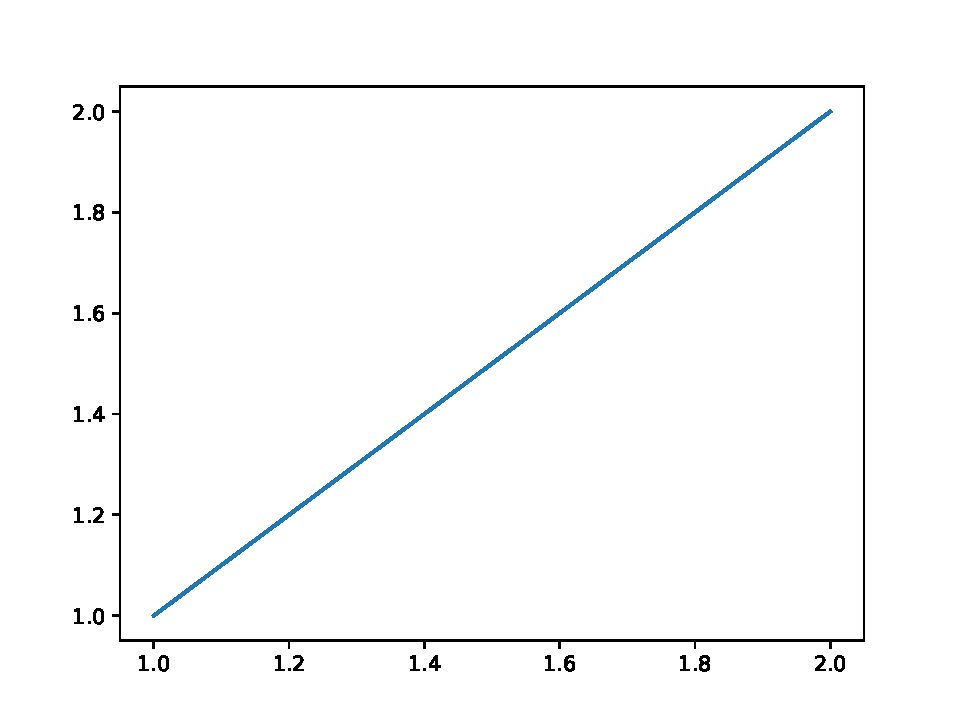
\includegraphics[width=\textwidth]{figs/nsw_curve.pdf}
  \caption{NSW over training steps (mean$\pm$CI).}
  \label{fig:nsw_curve}
\end{subfigure}
\hfill
\begin{subfigure}[t]{0.48\textwidth}
  \centering
  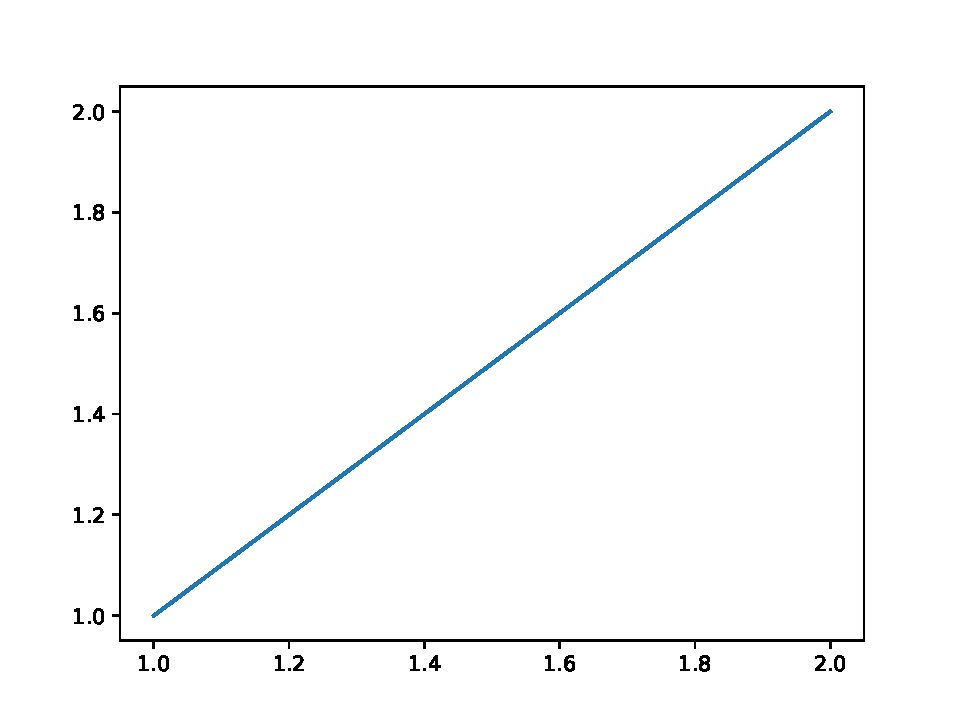
\includegraphics[width=\textwidth]{figs/gini_curve.pdf}
  \caption{Gini over training steps (mean$\pm$CI).}
  \label{fig:gini_curve}
\end{subfigure}
\caption{Learning curves. CSC improves NSW while reducing inequality.}
\label{fig:learning_curves}
\end{figure}

\subsection{Ablations and deviation robustness}
\label{sec:ablations}

\Cref{tab:ablation_results} shows that removing AVoI, KL grounding, or arbitration degrades at least one axis among equity, robustness, and deviation resistance.

\begin{table}[t]
\centering
\caption{\textbf{Ablations and deviation robustness.} SDR/DVR definitions: Appendix~\ref{app:metrics}.}
\label{tab:ablation_results}
\begin{tabular}{lcccc}
\toprule
Variant & Gini $\downarrow$ & Res. AUC $\uparrow$ & SDR $\downarrow$ & DVR $\downarrow$ \\
\midrule
CSC (Full)      & \todo{} & \todo{} & \todo{} & \todo{} \\
w/o AVoI        & \todo{} & \todo{} & \todo{} & \todo{} \\
w/o KL          & \todo{} & \todo{} & \todo{} & \todo{} \\
w/o Arbitration & \todo{} & \todo{} & \todo{} & \todo{} \\
\bottomrule
\end{tabular}
\end{table}

\subsection{Shock and Byzantine robustness}
\label{sec:robustness}

\Cref{fig:resilience_heatmap} visualizes resilience across shock parameters.
Full sweep grids and Byzantine heatmaps appear in Appendix~\ref{app:shock} and Appendix~\ref{app:byzantine}.

\begin{figure}[t]
\centering
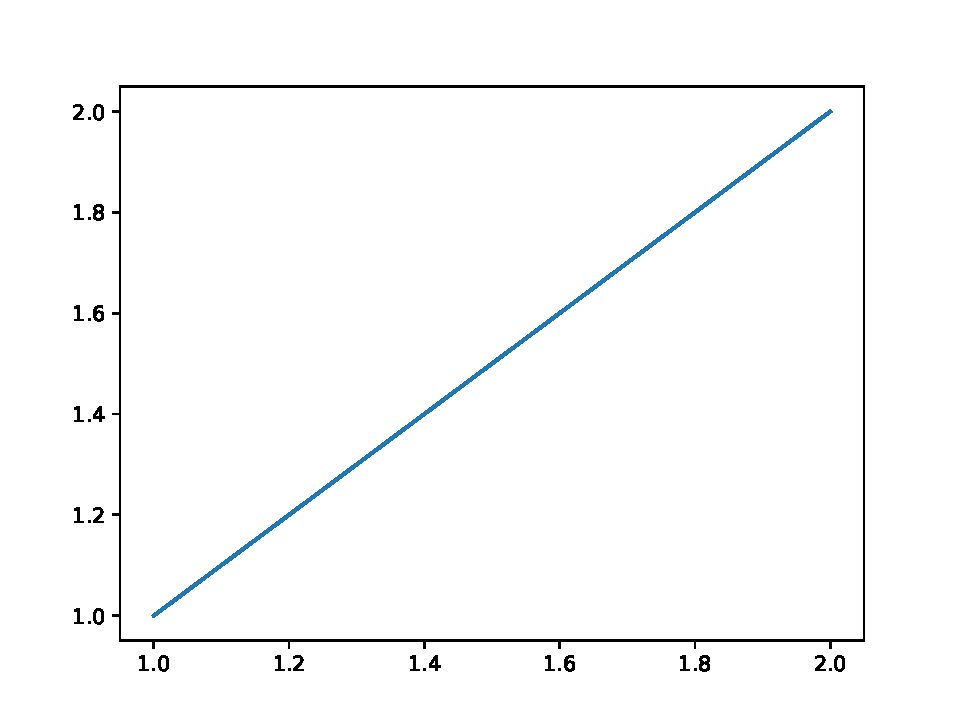
\includegraphics[width=0.78\textwidth]{figs/resilience_heatmap.pdf}
\caption{Resilience under resource shocks (survival probability). Full grids and AUC computation: Appendix~\ref{app:shock}.}
\label{fig:resilience_heatmap}
\end{figure}

% =========================================================
\section{Discussion and Limitations}
\label{sec:discussion}

\paragraph{Scope control.}
All claims are restricted to Markov-game collectives splitting finite resources and do not assume human-level semantics.

\paragraph{Limitations.}
\textbf{Welfare choice:} NSW discourages near-zero outcomes but can be sensitive when returns approach zero; we stabilize with $\epsilon$ and report Gini/Jain.
\textbf{Masking realism:} AVoI assumes identity signals can be suppressed during contract learning; partial/noisy variants mitigate but do not eliminate this constraint.
\textbf{Enforcement:} arbitration depends on detector calibration; we fix FPR and report ROC/AUC (Appendix~\ref{app:detector}), but formal auditing guarantees remain open.
\textbf{Scaling:} arbitration introduces overhead; scaling and wall-clock are reported in Appendix.

% =========================================================
\section{Conclusion}
\label{sec:conclusion}

We presented \textbf{Computational Social Contract (CSC)}, a protocol for collective alignment in heterogeneous multi-agent systems.
CSC learns a symmetric contract under an Algorithmic Veil of Ignorance and stabilizes identity-aware execution via KL grounding and arbitration trained against evasive deviations.
On \textit{Silicon Commune}, CSC improves equity and robustness with competitive efficiency.

% =========================
% References
% =========================
\bibliographystyle{plainnat}
\bibliography{refs}

% =========================================================
% Appendix
% =========================================================
\appendix

\section{Metric Definitions}
\label{app:metrics}

\subsection{Throughput and Returns}
We report system throughput as total realized extraction per episode:
\[
\mathrm{Throughput}=\sum_{t=1}^T \tilde{E}_t.
\]
Episodic return:
\[
G_i=\sum_{t=1}^T \gamma^{t-1} r^{shaped}_{i,t}.
\]

\subsection{Nash Social Welfare (NSW)}
We use an $\epsilon$-stabilized form:
\[
\NSW(\pi)=\frac{1}{n}\sum_{i=1}^n \log\left(\E_\pi[G_i]+\epsilon\right),
\quad \epsilon=10^{-3}.
\]

\subsection{Gini and Jain}
Gini:
\[
\mathrm{Gini}(x)=\frac{\sum_{i=1}^n\sum_{j=1}^n |x_i-x_j|}{2n^2 \bar{x}+\epsilon_G},
\quad \bar{x}=\frac{1}{n}\sum_i x_i.
\]
Jain:
\[
\mathrm{Jain}(x)=\frac{(\sum_{i=1}^n x_i)^2}{n\sum_{i=1}^n x_i^2+\epsilon_J}.
\]

\subsection{Collapse and Resilience}
Collapse:
\[
\text{Collapse} \iff \exists t \le \alpha T:\ R_t \le \epsilon_R,
\quad \alpha=0.3,\ \epsilon_R=10^{-3}.
\]
Resilience:
\[
\mathrm{Resilience}=\Pr[\neg \text{Collapse}].
\]
Resilience AUC averages survival over a parameter grid (Appendix~\ref{app:shock}).

\subsection{DVR and SDR}
DVR:
\[
\mathrm{DVR}=\frac{1}{nT}\sum_{i=1}^n\sum_{t=1}^T \ind[d_\omega(o_{i,t},a_{i,t})\ge \tau].
\]
SDR uses paired rollouts with shared randomness over a deviation window $H$:
\[
\Delta G_i(t,H)=G_i^{dev}(t,H)-G_i^{contract}(t,H),
\quad \mathrm{SDR}=\frac{\#\{(i,t):\Delta G_i(t,H)>\delta\}}{\#\{(i,t)\}}.
\]

% ---------------------------------------------------------
\section{Shock Sweeps and Resilience AUC}
\label{app:shock}

\subsection{Shock families}
We evaluate three shock families:
(i) Bernoulli shocks with $(p_{shock}, s_{shock})$;
(ii) Poisson shocks with $(\lambda, s_{shock})$;
(iii) Markov shocks with $(p_{01}, p_{10}, s(1))$.

\subsection{Sweep grids}
Bernoulli:
\[
p_{shock}\in\{0.0,0.05,0.10,0.20,0.30\},\quad
s_{shock}\in\{0.1,0.3,0.5,0.7\}.
\]
Poisson:
\[
\lambda\in\{0.0,0.05,0.10,0.20,0.30\},\quad
s_{shock}\in\{0.1,0.3,0.5,0.7\}.
\]
Markov:
\[
p_{01}\in\{0.02,0.05,0.10\},\quad
p_{10}\in\{0.05,0.10,0.20\},\quad
s(1)\in\{0.3,0.5,0.7\}.
\]

\subsection{AUC computation}
\[
\mathrm{AUC}=\frac{1}{|\Theta|}\sum_{\theta\in\Theta}\mathrm{Resilience}(\theta).
\]

% ---------------------------------------------------------
\section{Byzantine Stress Tests}
\label{app:byzantine}

Let $\mathcal{B}$ denote Byzantine agents with fraction $f_B=|\mathcal{B}|/n$.
A Byzantine agent executes an attack policy with probability $\pi_B$ and follows the nominal policy otherwise.
We evaluate greedy hoarding ($a\equiv 1$) and learned proposer deviations (Appendix~\ref{app:detector}).

% ---------------------------------------------------------
\section{Detector Calibration and ROC/AUC}
\label{app:detector}

\subsection{Training data}
We collect (i) contract samples from $\pi_{\text{contract}}$ labeled $y=0$ and (ii) deviation samples from proposer $q_\psi$ labeled $y=1$.
Detector is trained with balanced BCE.

\subsection{Threshold calibration}
We select $\tau$ by fixing a target FPR on contract-only data:
\[
\tau = \min\left\{t:\Pr(d_\omega(o,a)\ge t \mid y=0)\le \mathrm{FPR}^\star\right\},
\quad \mathrm{FPR}^\star=0.05.
\]
We report ROC/AUC \citep{fawcett2006roc}.

% ---------------------------------------------------------
\section{Silicon Commune Environment}
\label{app:env}

\subsection{Dynamics (pseudocode)}
\begin{algorithm}[H]
\caption{Silicon Commune Step (pseudocode)}
\label{alg:commune_step}
\begin{algorithmic}[1]
\STATE Inputs: resource $R_t$, endowments $(c_i,m_i)$, actions $a_{i,t}$
\STATE Attempted extraction $E_t \leftarrow \sum_i m_i a_{i,t}$
\STATE Realized extraction $\tilde{E}_t \leftarrow \min(R_t, E_t)$
\FOR{$i=1..n$}
  \STATE Allocation $e_{i,t} \leftarrow \tilde{E}_t \cdot \frac{m_i a_{i,t}}{\sum_j m_j a_{j,t}+\epsilon_E}$
  \STATE Utility $u_{i,t}\leftarrow \log(1+c_i e_{i,t})$
  \STATE Reward $r_{i,t}\leftarrow u_{i,t}-\lambda_c\cdot \mathrm{cost}(a_{i,t})$
\ENDFOR
\STATE Apply shock $\xi_t$ (Appendix~\ref{app:shock}); update $R_{t+1}\leftarrow \max\{0, R_t-\tilde{E}_t+\rho-\xi_t\}$
\STATE Shape reward via detector (Eq.~\ref{eq:shaping})
\end{algorithmic}
\end{algorithm}

% ---------------------------------------------------------
\section{Hyperparameter Search}
\label{app:hparam_search}

We match interaction budgets across methods and run an equal number of trials.
We select by validation NSW (or total return when NSW is unavailable).

% ---------------------------------------------------------
\section{Reproducibility Checklist}
\label{app:repro}

We will release:
(i) environment code,
(ii) training and evaluation configs,
(iii) all random seeds and sweep scripts,
(iv) raw logs for all runs,
(v) pretrained checkpoints for main models.

\end{document}
